%You can delete all the comments after you have finished your document
%this sets up the defaults for the documents, 12pt font and A4 size. The article type sets this up as such as opposed to letter or memo.

%for the finer points LaTeX see https://en.wikibooks.org/wiki/LaTeX or http://tex.stackexchange.com/

\documentclass[12pt,a4paper]{article}
\usepackage{titlesec} %these are how we import packages, one helps set up footers and title layout
\usepackage{fancyhdr}

% !TEX TS-program = pdflatex
% !TEX encoding = UTF-8 Unicode
\usepackage[utf8]{inputenc} % set input encoding (not needed with XeLaTeX)

\usepackage{graphicx} % support the \includegraphics command and options
\graphicspath{{./appendicies/}}

% \usepackage[parfill]{parskip} % Activate to begin paragraphs with an empty line rather than an indent

%%% PACKAGES
\usepackage{booktabs} % for much better looking tables
\usepackage{array} % for better arrays (eg matrices) in maths
\usepackage{paralist} % very flexible & customisable lists (eg. enumerate/itemize, etc.)
\usepackage{verbatim} % adds environment for commenting out blocks of text & for better verbatim
\usepackage{subfig} % make it possible to include more than one captioned figure/table in a single float
\usepackage[toc,page]{appendix}
\usepackage{apalike}
% These packages are all incorporated in the memoir class to one degree or another...

\newcommand{\figuremacro}[5]{
    \begin{figure}[#1]
        \centering
        \includegraphics[width=#5\columnwidth]{#2}
        \caption[#3]{\textbf{#3}#4}
        \label{fig:#2}
    \end{figure}
}

%header and footer settings
\pagestyle{fancyplain}
\fancyhf{}
\renewcommand{\headrulewidth}{0.5pt}
\renewcommand{\footrulewidth}{0.5pt}
\setlength{\headheight}{15pt}
\fancyhead[L]{Dylan Tyrie-Dron - 40203045}
\fancyhead[R]{ SOC10101 Honours Project}
\fancyfoot[L]{}
\fancyfoot[C]{\thepage}

%set better section layout
\makeatletter
\renewcommand\subsection{\@startsection {subsection}{1}{2mm} % name, level, indent
                               {3pt plus 2pt minus 1pt} % before skip
                               {3pt plus 0pt} % after skip
                               {\normalfont\bfseries}}
\makeatother
\makeatletter
\renewcommand\section{\@startsection {section}{1}{0mm} % name, level, indent
                               {4pt plus 2pt minus 1pt} % before skip
                               {4pt plus 0pt} % after skip
                               {\bfseries}}
\makeatother


%this starts the document
\begin{document}

%you can import other documents into your main one, these layout the Title and Declarations on its own page.
%you might need to change these to \ if your on Microsoft Windows.
\newcommand{\HRule}{\rule{\linewidth}{0.5mm}}

\begin{titlepage}
	\begin{center}

	\HRule \\[0.4cm]
    	{\Large \bfseries Adaptation of a Satellite Navigation System\par}
	\vspace{0.2cm}
	\HRule \\[1.5cm]

	
    	\vspace{3cm}
	\begin{minipage}{0.4\textwidth}
	\begin{center} \large
        \emph{}\\
        	Dylan Tyrie-Dron - 40203045
				
   	 \end{center}
    	\end{minipage}
	
	\vspace{2cm}
    	\begin{minipage}{1\textwidth}
    	\begin{center} \large
        
		Submitted in partial fulfilment of \\
		the requirements of Edinburgh Napier University \\
		for the Degree of \\
        	BEng (Hons) Software Engineering
    	\end{center}
    	\end{minipage}

    	\vfill

    	% Bottom of the page
	\begin{minipage}{1\textwidth}
    	\begin{center} \large
		School of Computing
    	\end{center}
    	\end{minipage}
	
	\vspace{1cm}
    	{\large \today}


	\end{center}
\end{titlepage}
%{\large Submitted in partial fulfilment of the requirements of Edinburgh Napier University for the Degree of }

\section*{Authorship Declaration}
\vspace{0.5cm}
\begin{flushleft}
I, (Dylan Tyrie-Dron), confirm that this dissertation and the work presented in it are my own achievement.\newline

Where I have consulted the published work of others this is always clearly attributed;\newline

Where I have quoted from the work of others the source is always given. With the exception of such quotations this dissertation is entirely my own work;\newline

I have acknowledged all main sources of help; \newline

If my research follows on from previous work or is part of a larger collaborative research project I have made clear exactly what was done by others and what I have contributed myself;\newline

I have read and understand the penalties associated with Academic Misconduct.\newline

I also confirm that I have obtained informed consent from all people I have involved in the work in this dissertation following the School's ethical guidelines.\newline
\end{flushleft}

\begin{flushleft} \large
\emph{Signed:} \\
\end{flushleft}

\vspace{.5cm}

\begin{flushleft} \large
\emph{Date:} \\
\end{flushleft}

\vspace{.5cm}

\begin{flushleft} \large
\emph{Matriculation no: }  \\
\end{flushleft}
\pagebreak

\section*{General Data Protection Regulation Declaration}
\vspace{0.5cm}
\begin{flushleft}
Under the General Data Protection Regulation (GDPR) (EU) 2016/679, the University cannot disclose your grade to an unauthorised person. However, other students benefit from studying dissertations that have their grades attached. \newline

\vspace{0.5cm}

Please sign your name below one of the options below to state your preference.\newline
\vspace{0.5cm}

The University may make this dissertation, with indicative grade, available to others.\newline
\vspace{3cm}


The University may make this dissertation available to others, but the grade may not be disclosed.\newline
\vspace{3cm}


The University may not make this dissertation available to others.\newline
\end{flushleft}



\pagebreak

%LaTeX let you define the abstract separately so it wont get sucked into the main document.
\begin{abstract}
% fill the abstract in here
\end{abstract}
\pagebreak

\tableofcontents % is generated for you
\newpage

\listoftables
%generated in same way as figures
\newpage

\listoffigures
%you may have captions such as equations, listings etc they should all appear as required
%these are done for you as long as you use \begin{figure}[placement settings] .. bla bla ... \end{figure}
\newpage

\section*{Acknowledgements}
Insert acknowledgements here
\subsection*{}
	I would like to thank my cat, dog and family.
\newpage


\section{Introduction}
The aim of this project is to describe a way of navigating through a city through the use of real-time traffic data. This will be achieved by testing different pathfinding algorithms for example: \cite{Dijkstra1959}. Research will also be carried out on traffic and other data affecting vehicles getting to their destinations faster. This will be done by rigorously testing car speeds at certain times in the same place within the city Edinburgh. This should give data that can input into a pathfinding algorithm. The results will then be compared to similar experiments developed by others as a way of finding out which method was the most accurate, cost-effective and efficient to travel through a city and discussing which methods are the most suitable for getting through any city. The main interface used to convey the outcome of this project is an android application. It is also thought to make use of API’s like: “OpenstreetMaps” to speed up the development.


\section{Literature Review}

\subsection{Traffic Research}
Traffic

\subsubsection{}Some conditions for road users that affect the speed of cars and therefore traffic: road weather changes, car accidents and traffic congestion. \cite{Zheng2018}
\subsubsection{}Difference between distance based navigation (a) and time based navigation based navigation (b). As you can see the time based navigation works out that though the distance is greater for a car to travel from points 1-5 it takes less time than from points 1-3-5. (pic)
\subsubsection{}To find traffic congestion, find cars within one road or a set of roads that are averaging the lowest average speed and put the cars on different routes (repeat process) until the average speed has been brought up again to a more suitable average speed (20 km/h). \cite{Zheng2018}

\paragraph{}
 Equation to determine the speed weighting for cars in the current area: (cars in average speed cluster) / (total number of cars) * (average speed of cars in the current area). (equation) \cite{Zheng2018}
\subsubsection{}Traffic congestion is measured by detecting the average speed of the vehicles and if the vehicles are moving slower than 10km/h, then a road is congested \cite{DAndrea2017}.

\subsection{Google Maps}
Google maps was introduced in 2005, revolutionising the way maps worked when display on websites as it allowed users to interact with the map \cite{Svennerberg2010}.
\subsubsection{Google Maps Elevation API}
Google Maps allows users to see the elevation of locations through the "terrain layer". This layer shades in different parts of the map to show which locations are higher than others. This data is taken from the "Elevation API". This allows users of the API to find the elevation of certain locations by providing the "LocationElevationRequest" with a GPS coordinate which will in return provide the user with an elevation for that GPS coordinate in meters. This API also allows the user to request a set of GPS coordinates along a path by providing the "PathElevationRequest" with two or more GPS coordinates along a path along with a number of samples for the path to be split up into, for example if a the path had two GPS coordinates and was split up into 16 samples then the "PathElevationRequest" would return a graph with 16 elevations between the two coordinates specified \cite{googleElevation}.

\figuremacro{h}{googleElevationPath}{PathElevationRequest}{- This is what PathElevationRequest returns for 6 coordinates at 256 samples.}{1.0} 

\subsection{TomTom maps}
TomTom was founded in 1991 beginning in the business-to-business section of the technology market. They then went on to develop personal digital assistants (PDAS) in the early 90s, going on to become the market leader in PDA software with navigation applications such as "RoutePlanner" and "Citymaps". In 2002, the TomTom "Navigator" provided the first affordable and easy-to-use navigation system to customers in Europe.

This increased demand for portable navigation devices, which lead to the development of the Portable Navigation Device (PND). This became the fastest selling consumer technology device in history and by 2016 TomTom had sold over 78 million PNDs.

Nowadays, TomTom provide customers with several navigation-based products, including a navigation app for android and wrist devices for sports enthusiasts, reaching over 800 million people a day \cite{TomTomHist}.

\subsubsection{Map tiles}
The TomTom maps API provides the user to view the maps using raster tile images or vector tile images. The difference is subtle when viewing the maps, however in theory, raster tiles should be more detailed as the tile is coloured per pixel whereas vector imaging colours the tile based on the objects inside it (roads, rivers, etc.).

The number of tiles shown depends on the level of zoom that the user has defined (by using a pinching gesture on the screen). There are 23 different levels of zoom with 0 showing the whole world in one tile and zoom level 22 showing 2 to the power of 22 tiles. 

\figuremacro{h}{TomTomZoom1}{Zoom level 1}{- This is Zoom Level 1 which is 4 tiles in total.}{1.0} 

\subsubsection{Map layers}
The TomTom maps API also allows the maps to be separated into different layers to make it easier to update the map or to show places in different languages etc. There are three layers defined in the TomTom documentation: Basic, Hybrid and Labels. The Basic layer shows all the maps features as an end user would see it. The Hybrid layer is a step down from that as it takes the polygons that outline the birds eye view of the buildings so that the view of the map is focussed on the roads more. The Labels layer shows only the labels of the named places shown on the map in the position they would be in, in the Basic layer. The allows the developer to see places more clearly which allows the addition of places to be easier and also to check whether the names of the places are in the correct place and are spelt correct in their respective languages.

The map also has styles that affect the way that the layers are shown: main and night. The main style is more of a light theme where all the usual map colours are used, however, the night style will use colours that are not too intrusive to the user at night \cite{TomTomLayers}.

There are also some layers that are not directly related to the map, these include: traffic incident road highlighting,

\subsubsection{Traffic data}
TomTom maps provide a traffic data API to allow developers to use real-time traffic data that TomTom collects. The data is split up into traffic incidents and traffic flows. The Traffic incidents API allows the user to be informed of traffic jams due to road incidents that will affect the route that the user takes. The traffic flow API tracks the users speed on the routes that they are taking so that the next user can benefit from the road being used before them to provide them with more accurate routing and predicted travel times. The traffic incident API updates every 2 minutes to give the user (and the software) the chance to change their route in accordance to the latest traffic incident updates. The traffic flow API is updated every minute.

The traffic incident API will return information to the user and the system that details the impact of certain traffic incidents within the tile the user is currently in, or in fact along the route that the user is taking. 

\subsubsection{Traffic data}

\subsection{Routing Research}

\subsubsection{}
Data stored form real-time cars in database to affect the routing algorithm: long/lat, time stamps, driving speed and orientation (data uploaded four times a minute to the server). \cite{Zheng2018}

\subsubsection{}
Compare the routing algorithm time with other routing algorithms like: Heristic1 (time-based algorithm), Heristic2 (time-based algorithm), Dijkstra (distance-based). \cite{Zheng2018}

\subsubsection{}
Based on data in Beijing, 60\% of the total time is spent on intersections, although, 2.7\% of all the intersections were main intersections (400 intersections) and they took 18\% of the total intersection-time suggesting that a large proportion of the total intersection-time was wasted on main intersections. \cite{Liu}

\subsubsection{}
OpenStreetMap description: the map of an area (region, province, city, etc) is implemented as an oriented graph characterised by two main elements: nodes and ways.
\paragraph{}
Nodes represent important positions on the map identified by GPS coordinates (lat and long) corresponding to Points of interest (POIs), intersections, points of change in direction on the same road (curves), etc. Thus, between two nodes a linear segment is defined. Each node is associated with n id and with a list tags that describes the characteristics of the node. The number of nodes on a road depends on the type of road (typically urban roads are described with a higher amount of nodes with respect to highways).
\paragraph{}
Ways are ordered sets of nodes constituting open or closed polygons, representing possible paths from the start node to the end note. The nodes of a way are listed consecutively and this allows identifying stretches of consecutive roads. (ref) 

\subsubsection{}
here is picture explaining the different types of segments(description of each needed before pic)
(pic)

\subsubsection{}
Graphhopper puts the base node (where the car starts) into both forwards and backwards lists (two opposite-direction lists that display nodes that the car has passed) until the second GPS reading is taken and then removes the nodes from list that is not needed after the second reading is put into the right list. (ref)

\subsubsection{}
The usual states of traffic that popular systems implement are: flowing, slow, very slowed and blocked. Another state was added by (ref) which is absent. Which means there is either no traffic or a total absence of vehicles, this is used for incident detection. The usual traffic systems will check the number of vehicles that have crossed a segment in an amount of time.

\subsubsection{}
In the (ref) the system checks if there is sufficient vehicles on each road segment and sets the traffic states based on a few rules:
\paragraph{}
- If there is insufficient vehicles:
If there is 0 vehicles then set state to absent
else then set the state to flowing

\paragraph{}
Else (if there is enough vehicles)
  Find the median speed of the cars in the road segment and compare the median speed to a percentage of the speed limit that is close enough to the actual speed limit.
  If the percentage of speed limit is reached (p1) or a higher speed is found, then set the traffic state to flowing.
  If it is within a set percentage range lower (p2) then the state is set to slower.
  If the speed is reaching an even lower percentage of the speed limit (p3) then the state is set to very slow.
  Else the traffic is blocked.
  In the experiments used in this paper: p1 = 50\% , p2 = 40\% and p3 = 30\% and the sufficient number of cars was set to 4.
  
  \subsubsection{}
  Google traffic takes account of four different traffic states: 
  (i) Normal speed of traffic (green colour)
  (ii) Slower traffic (yellow colour)
  (iii) Congestion (red colour)
  (iv) Blocked or stop-and-go traffic (dark red colour)

\subsection{Car average speed Research}

\subsubsection{Floating car data}
Problems with tracking average speed is that GPS is not entirely accurate. \cite{Jia}

Intersection delay is a factor that contributes to route calculation. \cite{Liu}
\subsection{Traffic sensor Research}
\subsubsection{RFID}
Disadvantages of active RFID: 
- Cost per tag
- Need for battery maintenance/ higher maintenance costs
- Higher probability of interfering with other devices using similar frequency bandwidths in the area (ISM networks)
- Propriety communication protocols

\paragraph{}
By contrast, advantages of passive RFID tags are:
- Theoretically, the obtained distance of seven meters based on static experiments in \cite{GarciaOya2018} is a good enough range for reading passive RFID tags as cars are normally just over two meters away from the pavement and based on the data rate (40Kbps- protocol: EPC GLOBAL 1G2 ISO 18000-6C) requires only twenty-five milliseconds to measure a tag. 
- In theory, the passive tag in this paper can measure cars passing at speeds of up  to one hundred kilometers an hour, which therefore suggests that for most use-cases in the city, cars can be read by passive tags.
- Another advantage is that the complex anti-collision protocol used in \cite{GarciaOya2018} is not necessary due to the reader, used in the experiments, being able to read multiple tags on the same plate.

The conclusion drawn from form this comparison is that the passive tag advantages outweigh the use of active tags, in this situation, as the active tags would be "overkill". These results are then validated by the car-in-motion sensor test results - at fifty kilomters an hour, ten tags were read in about 250 milliseconds. However, this approach is limited as the RFID reader needs constant \textit{or at least for the few seconds that a car passes the road sign with an RFID reader attached} line of sight with the car's RFID tag as anything such as a parked vehicle could block the reading. \cite{GarciaOya2018} 

\newpage
\bibliographystyle{apalike}
\bibliography{./diss}

%example of References. See https://en.wikibooks.org/wiki/LaTeX/Bibliography_Management
%might be good to use a separate document for these so your main work is not one really long text file. 

%you can crate this on a extra tex document just like the title or any other part of the document.
 \newpage
 \begin{appendices}
 \section{Project Overview}
 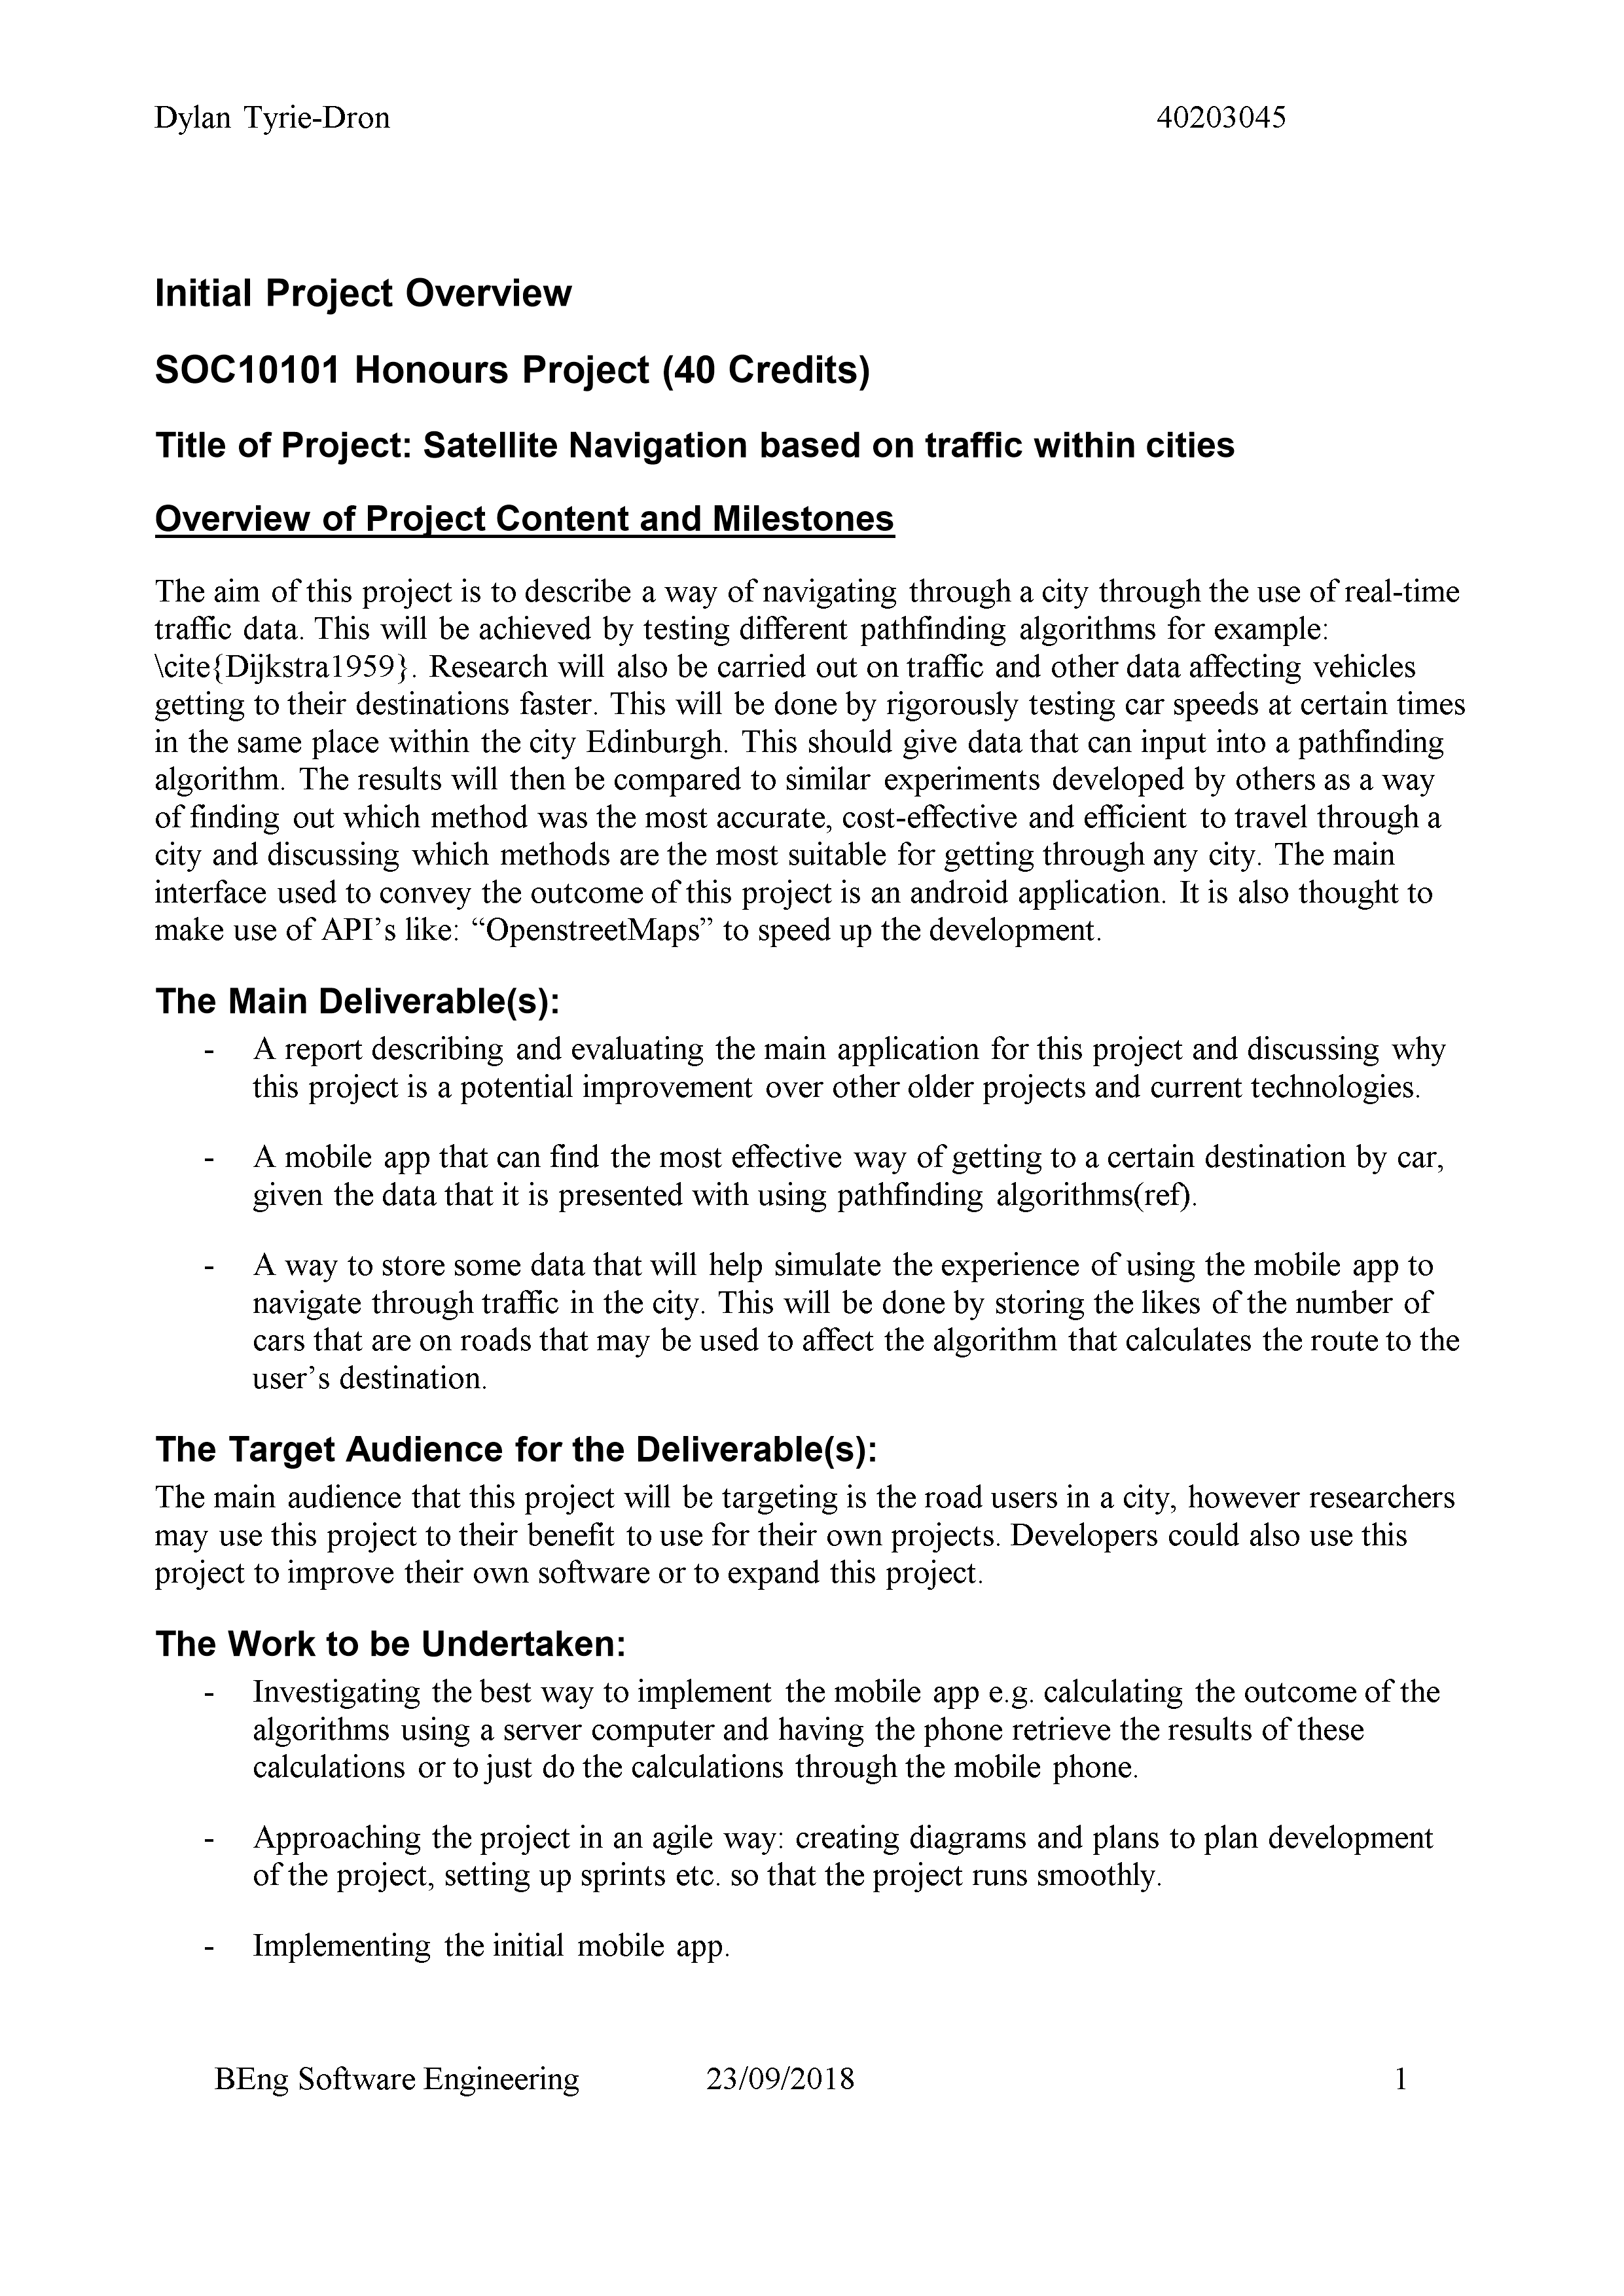
\includegraphics[width=\textwidth,height=\textheight,keepaspectratio]{IPOPage1.png} % fit images to page
\newpage
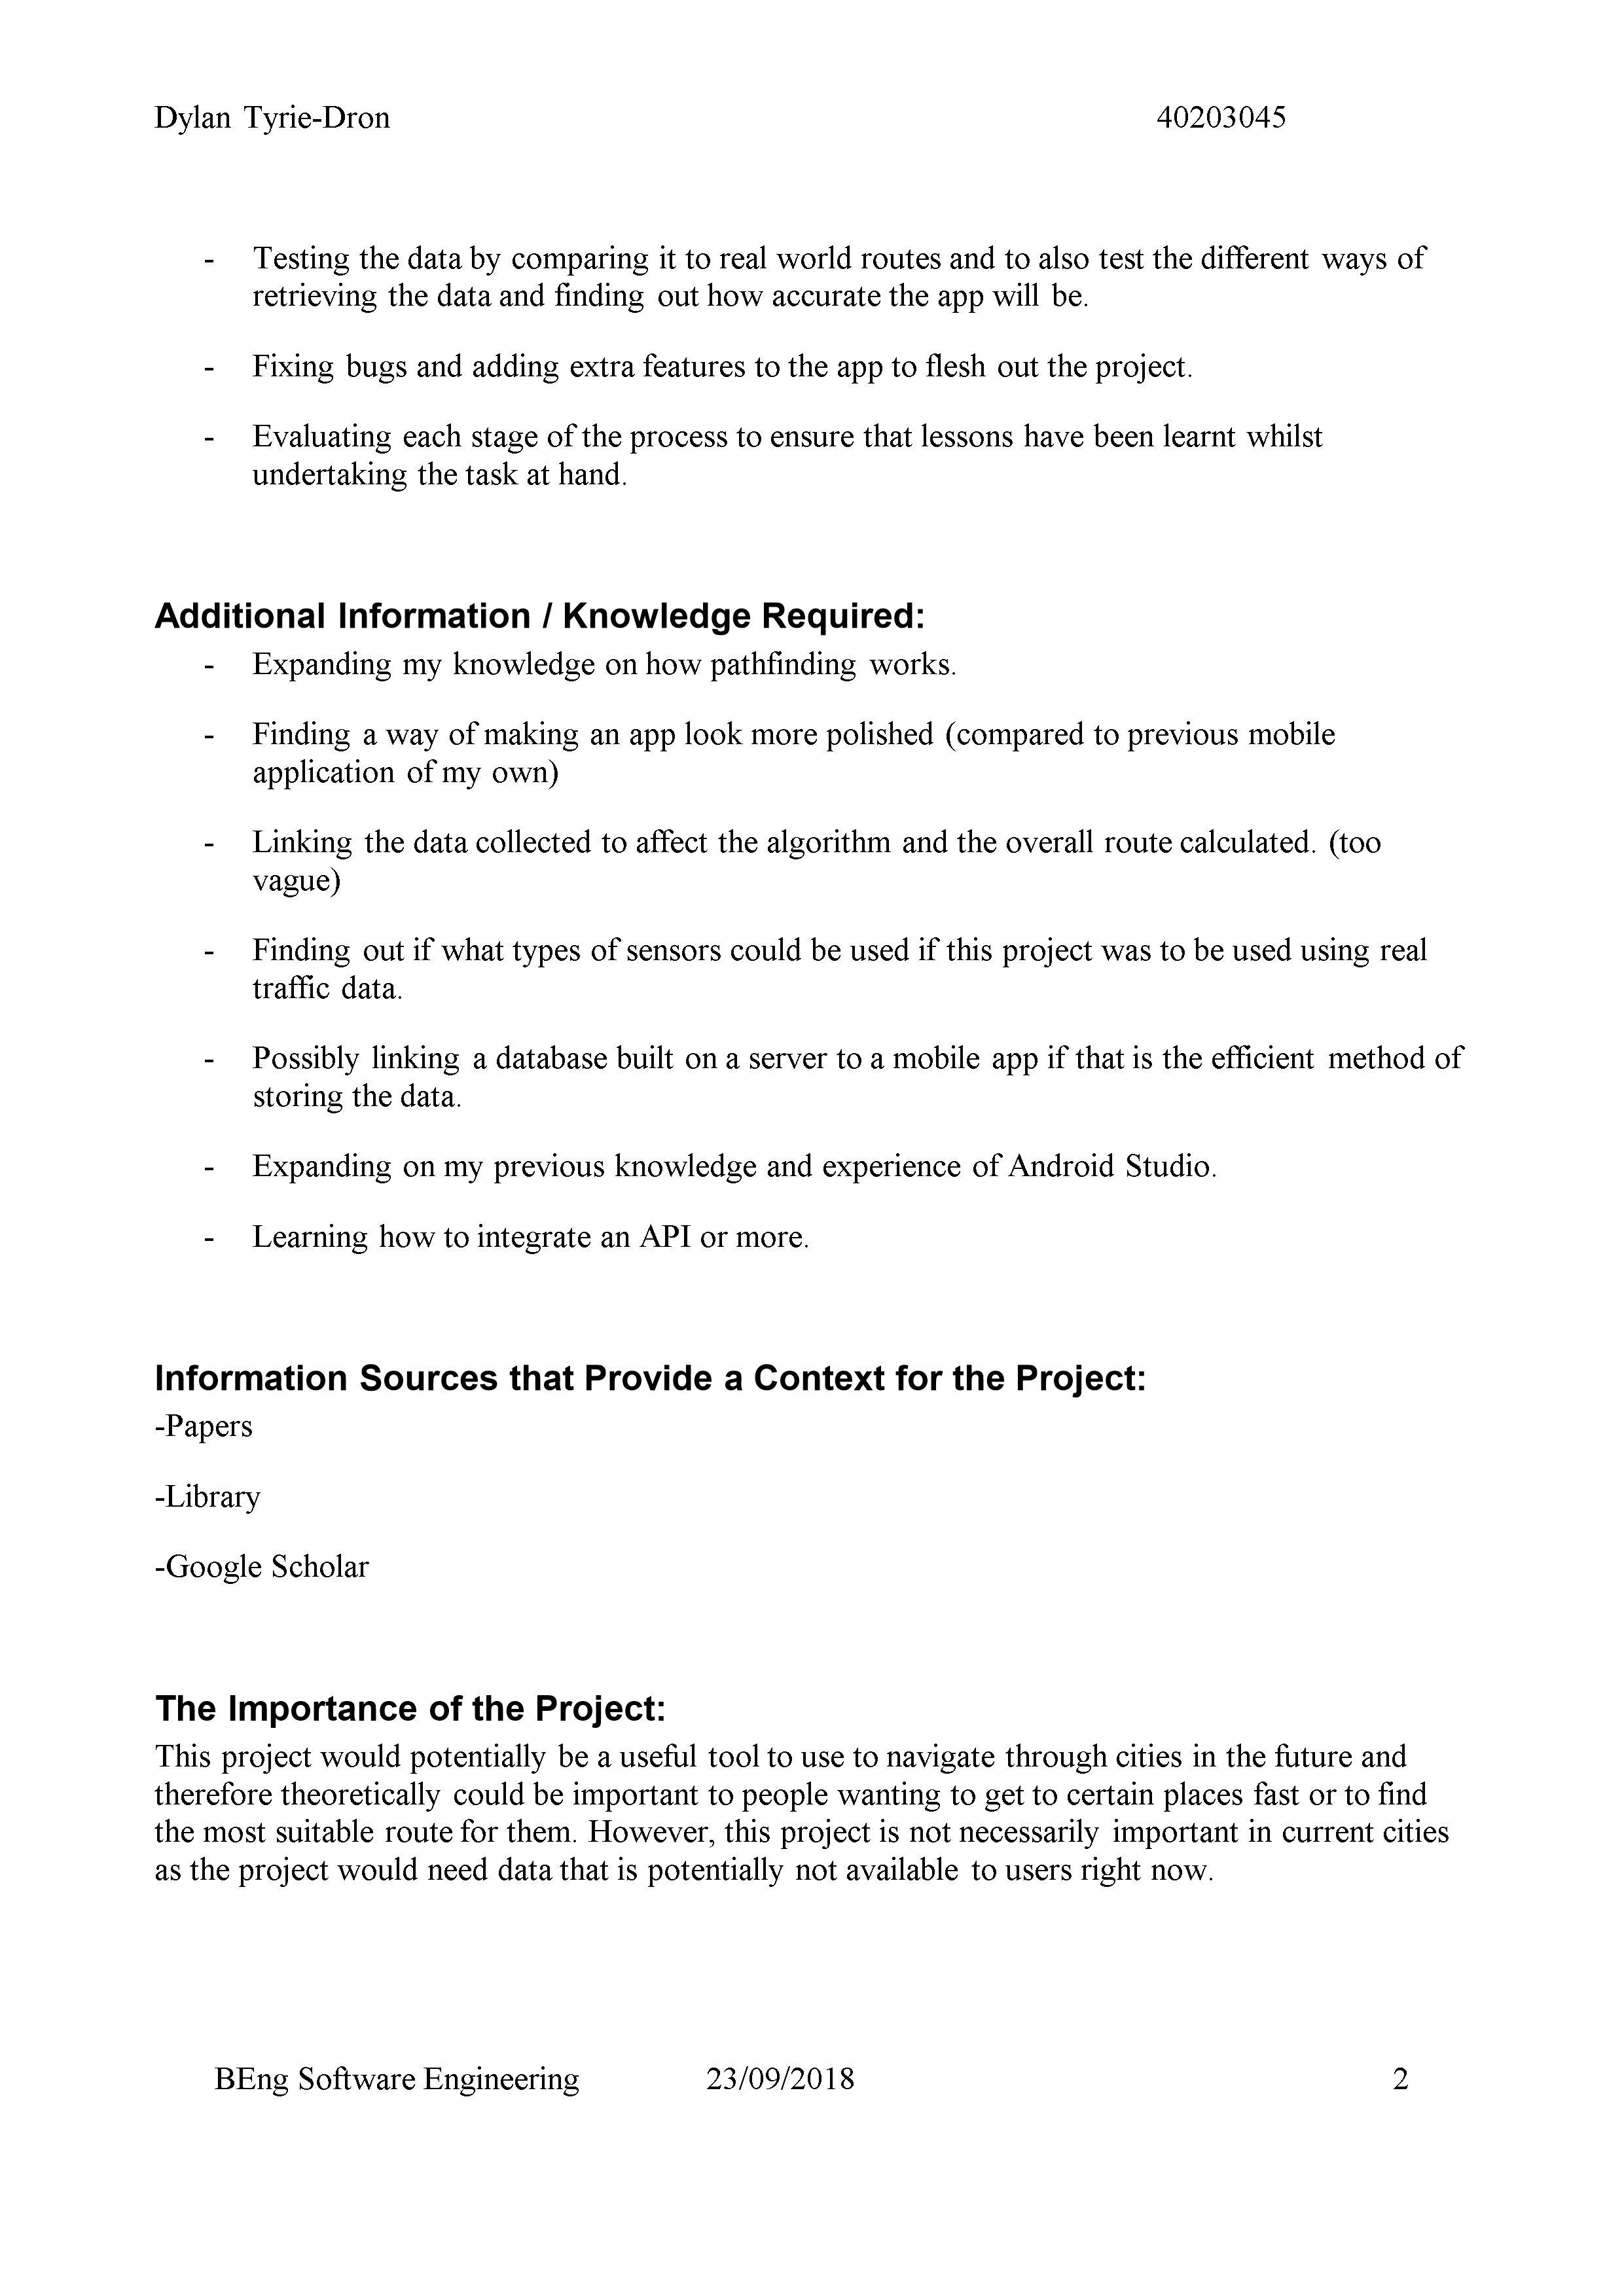
\includegraphics[width=\textwidth,height=\textheight,keepaspectratio]{IPOPage2.png}
\newpage

\includegraphics[width=\textwidth,height=\textheight,keepaspectratio]{IPOPage3.png} 
%insert IPO

% \begin{subappendices}
% \subsection{Example sub appendices}
% ...
% \end{subappendices}

% \section{Second Formal Review Output}
% Insert a copy of the project review form you were given at the end of the review by the second marker

 \section{Diary Sheets (or other project management evidence)}
% Insert diary sheets here together with any project management plan you have

\includegraphics[width=\textwidth,height=\textheight,keepaspectratio]{diary1.png} % fit images to page
\newpage
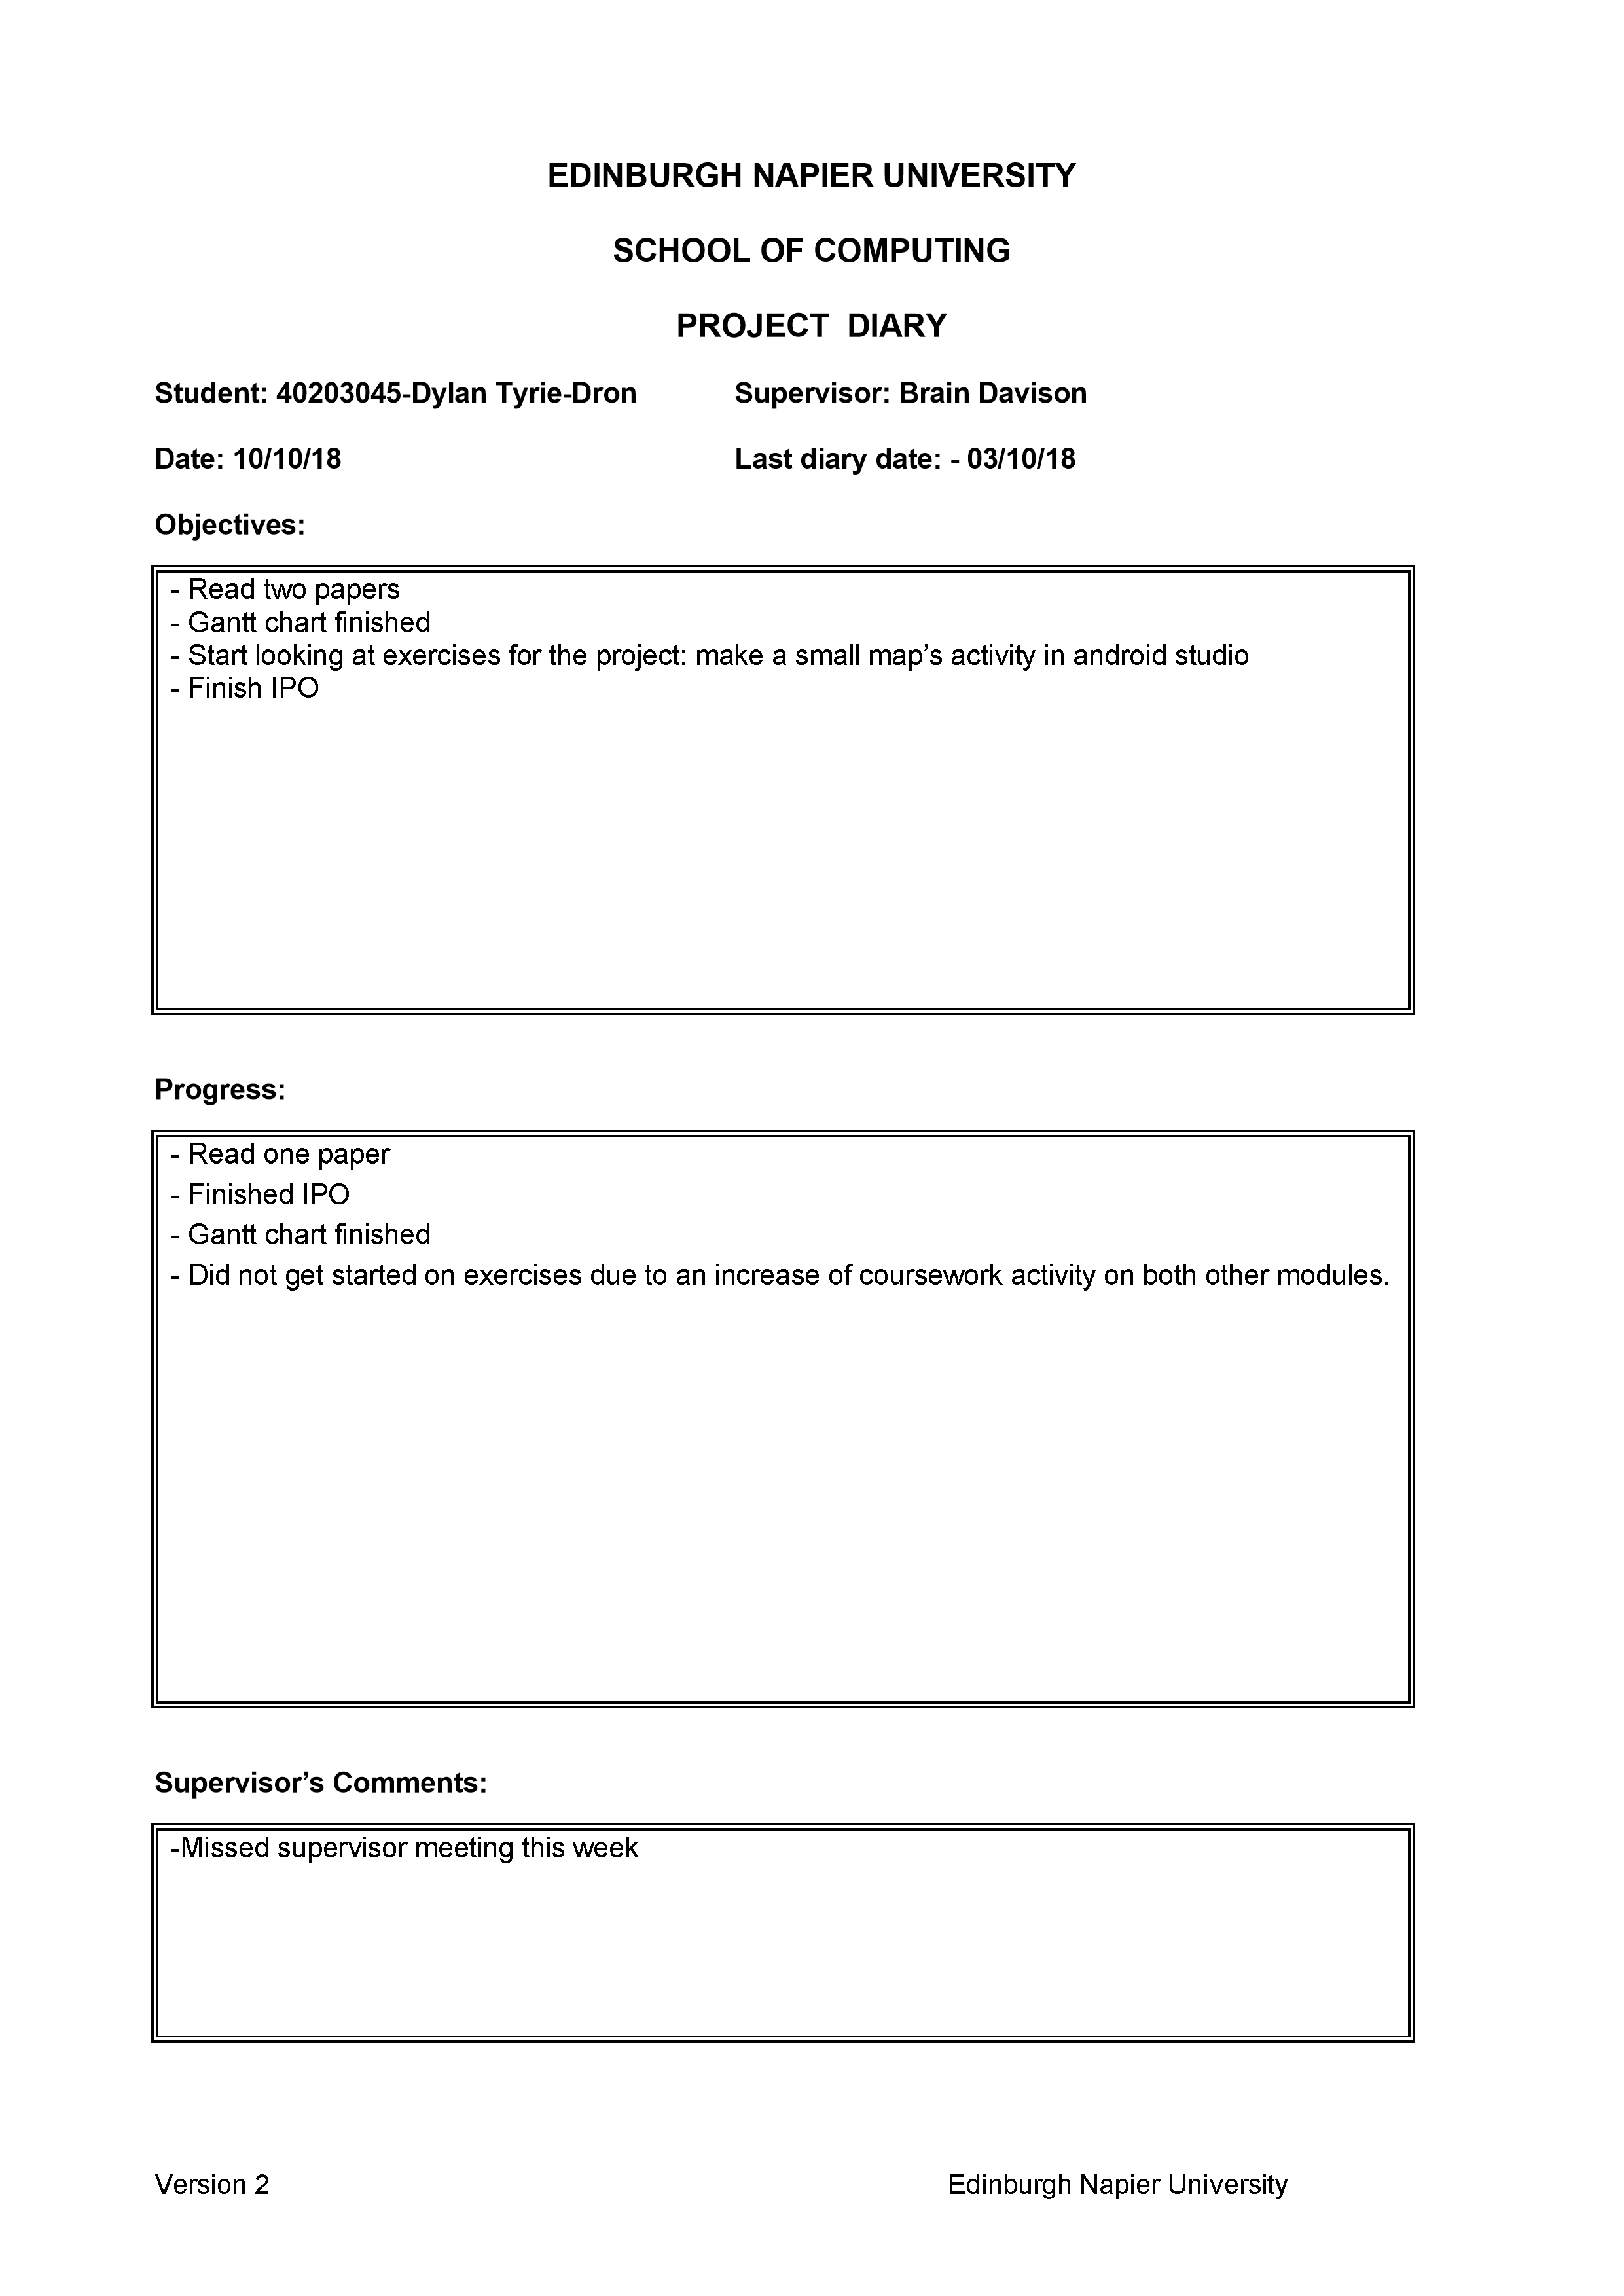
\includegraphics[width=\textwidth,height=\textheight,keepaspectratio]{diary2.png}
\newpage

\includegraphics[width=\textwidth,height=\textheight,keepaspectratio]{diary3.png} 
\newpage

\includegraphics[width=\textwidth,height=\textheight,keepaspectratio]{diary4.png} 
\newpage

\includegraphics[width=\textwidth,height=\textheight,keepaspectratio]{diary5.png}
% \section{Appendix 4 and following}
% insert content here and for each of the other appendices, the title may be just on a page by itself, the pages of the appendices are not numbered, unless an included document such as a user manual or design document is itself pager numbered.
 \end{appendices}

\end{document}
